\chapter{Theoretische Grundlagen}

Das Ziel dieser Arbeit besteht darin, ein Ersatzmodell für den Prototypen der 3D-Servo-Presse zu entwickeln. Die Parametrisierung erfolgt über Methoden des maschinellen Lernens. Auf Basis des Ersatzmodells folgt im weiteren Verlauf die Entwicklung von Konzepten zur Zustandsüberwachung und Regelung der 3D-Servo-Presse. Zunächst soll jedoch auf die Grundlagen der Modellbildung eingegangen werden.

\section{Modellierungsansätze}


Nach \cite{Isermann.2011} gibt es mehrere Möglichkeiten der Modellbildung, die theoretische, die experimentelle und theoretisch-experimentelle Mischformen. Zunächst erfolgt die Beschreibung der theoretischen Modellbildung. \\ 
Bei der theoretischen Modellierung findet die Beschreibung des Systems entweder über partielle oder gewöhnliche Differentialgleichungen statt. Da reale Systeme in vielen Fällen zu komplex und/oder kompliziert sind, ist es üblich, das Modell zu vereinfachen, z.B. durch das Ignorieren bestimmter real auftretender Effekte (z.B. nichtlineare Reibungseffekte). In der Regel ist es nach \cite{Isermann.2011} möglich, das Modell durch vier Arten von Gleichungen zu beschreiben:

\begin{itemize}
	
	\item \textit{Bilanzgleichungen:} Dazu gehören die Massen-, Energie- und Impulserhaltung.
	\item \textit{Physikalische oder chemische Zustandsgleichungen:} Diese sogenannten konstitutiven Gleichungen beschreiben reversible Vorgänge, wie z.B. das 2. Newtonsche Gesetz.
	\item  \textit{Phänomenologische Gleichungen:} Diese  beschreiben irreversible Vorgänge, wie z.B. Reibung.
	\item  \textit{Verbindungsgleichungen:} Dazu gehören die Kirchhoffschen Regeln, Momentengleichgewichte, etc.
	
\end{itemize} 

Nach \cite{Isermann.2011} setzt sich die theoretische Modellbeschreibung des Systems aus einer Mehrzahl von Gleichungen zusammen. Die Lösung des Gleichungssystems ist zwar explizit nicht immer möglich, aber trotzdem können individuelle Gleichungen wichtige Anhaltspunkte bezüglich der Modellstruktur liefern. \cite{Isermann.2011} \\
Die experimentelle Modellbildung basiert auf Messdaten, welche im Zuge von Versuchen aufgenommen werden. Die Messdaten teilen sich auf in Eingangs- und Ausgangsgrößen des Systems. Als Eingangsgrößen können entweder reale Eingangsstellgrößen oder künstlich erzeugte Testsignale mit bestimmten Eigenschaften fungieren. Im Fall der 3D-Servo-Presse seien der Exzentervorschub und die beiden Spindelvorschübe die Eingangsgrößen des Systems, da sie die Höhenverstellung des Stößels als Ausgangsgröße festlegen. Das Ziel der theoretischen Modellbildung besteht nun darin, für eine ausgewählte Modellstruktur die Parameter so zu identifizieren, dass ein möglichst guter Zusammenhang zwischen Eingangs- und Ausgangsgrößen hergestellt wird. Der dafür in der Literatur standardmäßig verwendete Begriff ist Systemidentifikation. \cite{Isermann.2011} \\
Die Bezeichnung der Modellstruktur, welche aus der theoretischen Modellbildung hervorgeht, lautet White-Box-Modell. Das Gegenstück dazu ist das Black-Box-Modell, welches aus der experimentellen Modellbildung hervorgeht. Nach \cite{Isermann.2011} haben White-Box- und Black-Box-Ansätze verschiedene Vor- und Nachteile, aber dennoch sind die komplementär zueinander. Um Vorteile beider Modellierungsansätze zu vereinen, sind ebenfalls sogenannte Gray-Box-Modell-Ansätze in verschiedenen Abstufungen (Light-Gray-Box-Modell, Dark-Gray-Box-Modell) entstanden. Eine Übersicht über alle Modellierungsansätze liefert Abbildung \ref{fig:modeling_methods}. Die wesentlichen Eigenschaften beider Modellierungsansätze sind in Tabelle \ref{tab:modeling_methods} zu finden. 




\begin{longtable}{p{7.0cm} p{7.0cm}}
	\caption{Eigenschaften theoretischer und experimenteller Modellierungsansätze \cite{Isermann.2011}} \\ \toprule
	% Definition des Tabellenkopfes auf der ersten Seite
	Theoretische Modellbildung & Experimentelle Modellbildung (Systemidentifikation) \\
	\hline
	\endfirsthead % Erster Kopf zu Ende
	% Definition des Tabellenkopfes auf den folgenden Seiten
	\caption{Lange Tabelle mit Longtable Fortsetzung}\\
	1 Spalte & 2 Spalte\\
	\hline
	\endhead % Zweiter Kopf ist zu Ende
	\hline
	
	% Ab hier kommt der Inhalt der Tabelle
	Modellstruktur folgt Naturgesetzen & Modellstruktur muss angenommen werden\\ \hline
	Modellierung des Übertragungsverhaltens und innerer Systemvorgänge & lediglich Identifizierung des Übertragungsverhaltens\\ \hline
	Gültigkeit des Modells für eine Reihe von Prozessen ähnlichen Types und unterschiedlicher Randbedingungen & Modell ist nur für das untersuchte System innerhalb der Betriebsgrenzen gültig\\ \hline
	Modellkoeffizienten sind nicht exakt bekannt & exaktere Bestimmung der Modellkoeffizienten für das gegebene System innerhalb der Betriebsgrenzen\\ \hline
	Modell kann für nicht existente Systeme entwickelt werden & Modell kann nur für ein bereits existierendes System entwickelt werden\\ \hline
	das interne Systemverhalten muss bekannt und mathematisch beschreibbar sein & Identifikationsmethoden sind unabhängig vom untersuchten System und können auf andere Systeme angewendet werden\\ \hline
	üblich langsamer Prozess mit hohem Zeitaufwand & schneller Prozess bei bereits bekannten Identifikationsmethoden\\ \hline
	Modelle können sehr komplex und detailliert ausfallen & Modellgröße kann auf den Anwendungsfall des Modells angepasst werden\\
	\bottomrule
	\label{tab:modeling_methods} 
\end{longtable}


\begin{figure} 
	\centering
	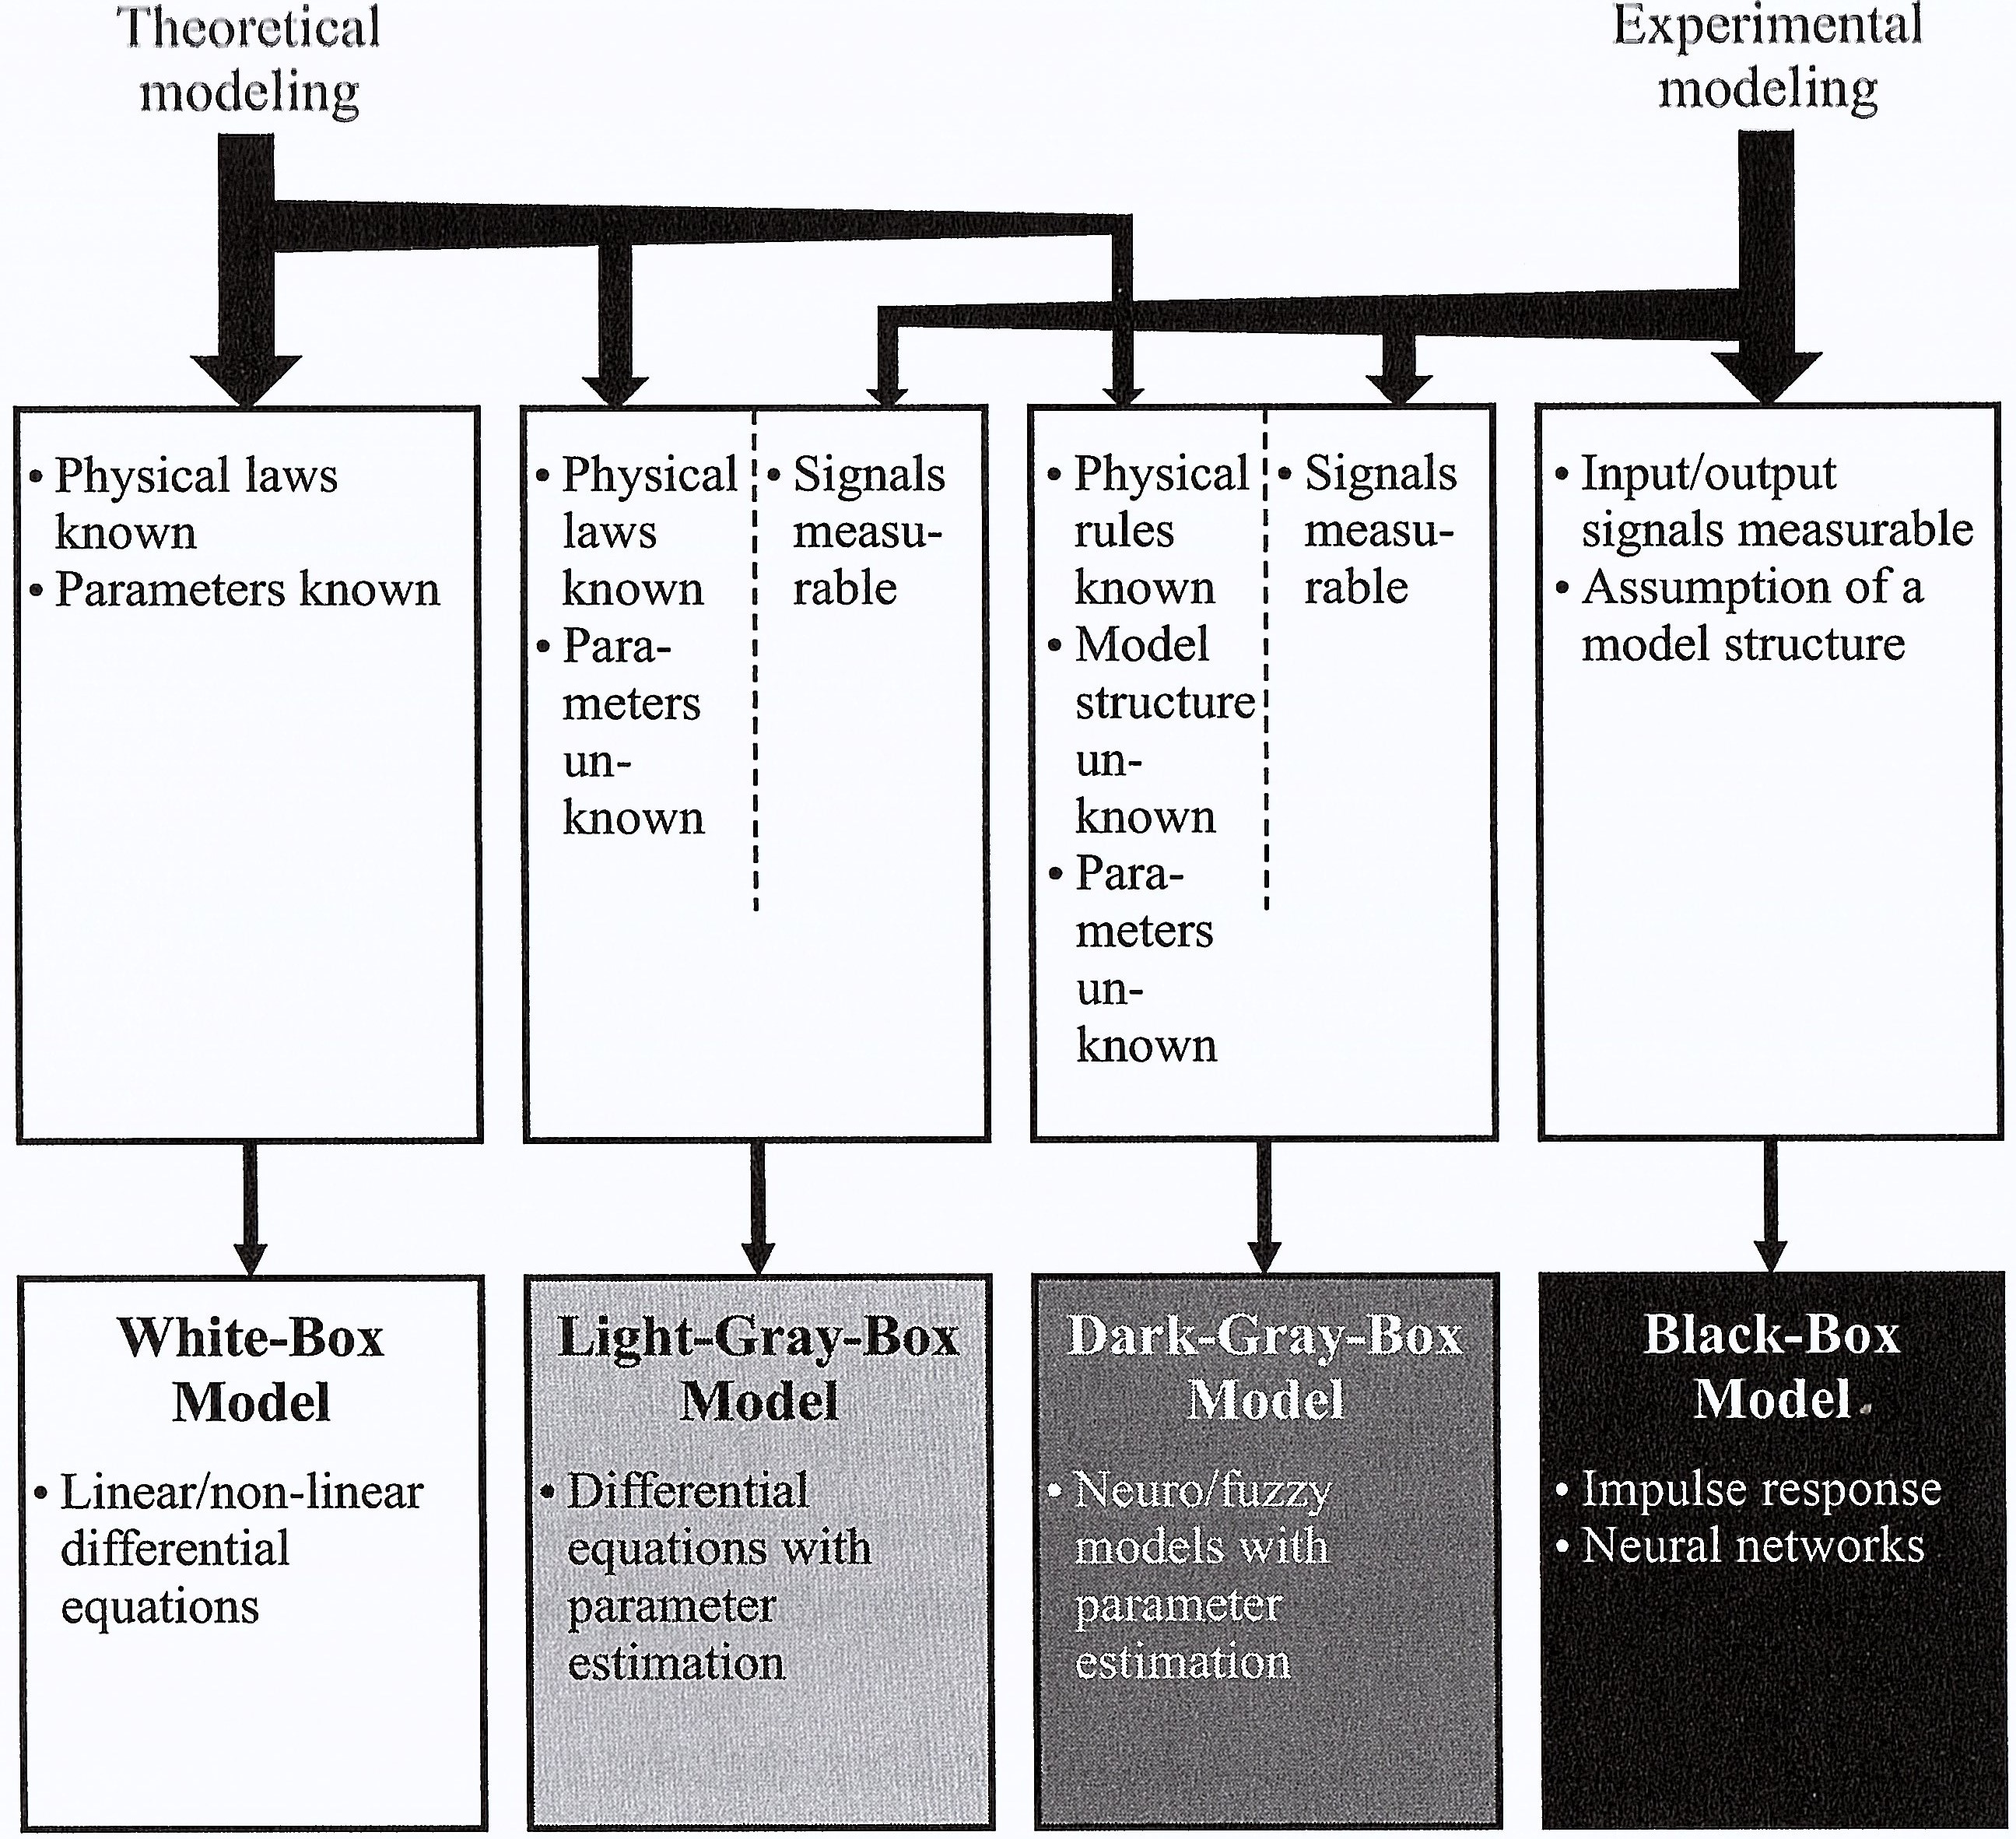
\includegraphics[width=0.75\textwidth]{images/modeling_methods}
	\caption{Verschiedene mathematische Modelle von White-Box- bis zu Black-Box-Modellen}
	\label{fig:modeling_methods}
\end{figure}

Wie in Tabelle \ref{tab:modeling_methods} zu erkennen ist, umgehen Black-Box-Modelle einen wesentlichen Nachteil von White-Box-Modellen, nämlich die exakte Kenntnis der Systemzusammenhänge, das Aufstellen von mathematischen Gleichungen zur Beschreibung dieser und die explizite Lösung des Gleichungssystems. Für komplexe Systeme  wie der 3D-Servo-Presse stößt der White-Box-Ansatz auf viele Probleme, siehe Abschnitt \ref{cha:Abgrenzung}. 
Deshalb fungiert das Black-Box-Modell als Grundlage für die Modellbildung des Prototypen der 3D-Servo-Presse.  Wie in Abbildung \ref{fig:modeling_methods} zu erkennen ist, können  Neuronale Netze als Methode zur Parameteridentifikation von Black-Box-Modellen dienen. Neuronale Netze stellen ein Teilgebiet des Maschinellen Lernens dar. Die Grundlagen der Neuronalen Netze werden in Kapitel QUELLE beschrieben. Das Black-Box-Modell dient als Grundlage für die Regelung und die Zustandsüberwachung der 3D-Servo-Presse. Zunächst sollen im nächsten Abschnitt die Grundlagen der Regelung vermittelt werden. 











